\documentclass[a4paper,12pt]{report}
\usepackage{amsmath}
\usepackage[english,russian]{babel}
\usepackage{framed}
\usepackage{graphicx}
\usepackage[utf8]{inputenc}

\graphicspath{{figures/}}
\DeclareGraphicsExtensions{.jpg}

% cчетчик программ, подчиненный счетчику глав
\newcounter{programcounter}[chapter]
% формат вывод счетчика программ
\renewcommand{\theprogramcounter}{\thechapter.\arabic{programcounter}}
% окружение для программ
\newenvironment{program}[1]
	{
		\medskip
		\refstepcounter{programcounter}
		\textit{Программа~\theprogramcounter. #1.}
		\ttfamily
		\begin{framed}
	}
	{
		\end{framed}
		\medskip
	}
% команда вывода строки программы со смещением
\newcommand{\programline}[2]{\noindent \hspace{#1em} #2 \par}
% команда вставки метки для программы
\newcommand{\programlabel}[1]{\label{program:#1}}
% команда вывода ссылки на программу с указанием номера
\newcommand{\programreference}[1]{программа~\ref{program:#1}}
% команда вывода ссылки на программу с указанием номера и страницы
\newcommand{\programreferencewithpage}[1]{программа~\ref{program:#1} на странице~\pageref{program:#1}}

\begin{document}

\title { Ускоренные методы умножения\\булевых матриц }
\author { Тигетов Давид }
\maketitle

\tableofcontents

\chapter { Введение }

В данном отчете рассматриваются различные методы умножения булевой матрицы $A$, имеющей порядок $n \times l$,
на булеву матрицу $B$, имеющей порядок $l \times m$, с размещением результата умножения в матрице $R$:
$$
	R = A \otimes B,
$$
$$
	\begin{pmatrix}
		r_{11} & r_{12} & \ldots & r_{1m} \\
		r_{21} & r_{22} & \ldots & r_{2m} \\
		\vdots & \vdots & \ddots & \vdots \\
		r_{n1} & r_{n2} & \ldots & r_{nm}
	\end{pmatrix}
 	=
	\begin{pmatrix}
		a_{11} & a_{12} & \ldots & a_{1l} \\
		a_{21} & a_{22} & \ldots & a_{2l} \\
		\vdots & \vdots & \ddots & \vdots \\
		a_{n1} & a_{n2} & \ldots & a_{nl}
	\end{pmatrix}
	\otimes
	\begin{pmatrix}
		b_{11} & b_{12} & \ldots & b_{1m} \\
		b_{21} & b_{22} & \ldots & b_{2m} \\
		\vdots & \vdots & \ddots & \vdots \\
		b_{l1} & b_{l2} & \ldots & b_{lm}
	\end{pmatrix}
$$

Для обозначения элементов матриц используются круглые скобки с номерами строки и столбца элемента, например,
$A(i,j)$ --- элемент $a_{ij}$ матрицы $A$:
$$
	A(i,j) = a_{ij}.
$$

Для обозначения строк и столбцов матриц используются те же круглые скобки, внутри которых один из номеров заменен
точкой $\cdot$, например, $A(i,\cdot)$ --- $i$-ая строка матрицы $A$:
$$
	A(i,\cdot) = ( a_{i1}, a_{i2}, \dots, a_{il} ).
$$

\chapter { Метод умножения строк на столцы }

\section { Описание метода }

В соответствии с определением умножения матриц каждый элемент $R(r,c)$ матрицы $R$ является результатом попарного умножения
элементов строки $A(r,\cdot)$ матрицы $A$ и элементов столбца $B(\cdot,c)$ матрицы $B$ с последующим сложением всех результатов
умножения:

$$
	R(r,c) = \bigoplus_{i=1}^{l} A(r,i) \otimes B(i,c)
$$

\chapter { Метод сложения строк } \label{section:RAM_row_addition_method}

\section { Описание метода } \label{section:RAM_description}

\marginpar{Нужен рисунок (формула не понятная)}
В соответсвии с правилом умножения каждая строка матрицы $R$ является линейной комбинацией (относительно операции
поэлементного сложения по модулю 2) строк матриц $B$, в которой множителями являются элементы строк матрицы $A$:
\begin{equation} \label{equation:RAMD_summing_by_rows}
	\forall r ( 1 \le r \le n ) : R(r,\cdot) = \bigoplus_{c=1}^{l} A(r,c) \otimes B(c,\cdot)
\end{equation}

\marginpar{И здесь нужен рисунок}
Аналогично столбцы матрицы $R$ можно вычислять путем суперпозиции столбцов матрицы $A$, в которой множителями
являются элементы столбцов матрицы $B$:
\begin{equation} \label{equation:RAMD_summing_by_columns}
	\forall c ( 1 \le c \le m ) : R(\cdot,c) = \bigoplus_{r=1}^{l} B(c,r) \otimes A(\cdot,r) 
\end{equation}

\section { Процедуры умножения }

Метод сложения строк, задаваемый общими соотношениями \ref{equation:RAMD_summing_by_rows} и
\ref{equation:RAMD_summing_by_columns}, допускает несколько различных вариантов организации вычислений,
оформленных в виде отдельных процедур умножения.

Приводимые далее описания указанных процедур умножения рассматриваются применительно к случаю вычисления матрицы $R$
по строкам, в соответствии с соотношением~\ref{equation:RAMD_summing_by_rows}, поскольку случай вычисления матрицы $R$ по
столбцам является аналогичным и не требует отдельного рассмотрения.

В соответствии с методом сложения строк требуется вычислять суммы строк матрицы $B$, причем в сумме, стоящей
справа в соотношении~\ref{equation:RAMD_summing_by_rows} некоторые элементы $A(r,c)$ матрицы $A$ могут оказаться
нулевыми, поэтому, вообще говоря, требуется складывать лишь те строки $B(c,\cdot)$ матрицы $B$, для которых
соответствующий элемент $A(r,c)$ равен единице. Отсюда происходят два различных подхода к вычислению сумм
строк матрицы $B$, которые разделяют процедуры умножения на две различные группы:
\begin{itemize}
	\item \emph{избирательные} процедуры, в которых производится анализ элементов матрицы $A$ и избирательное
			сложение строк матрицы $B$ для тех элементов $A(r,c)$, которые равны единице;
	\item \emph{массовые} процедуры, в которых всегда выполняется $l$ сложений, в которых участвуют все строки
			матрицы $B$, некоторые из которых "зануляются"{}, если соответствующий элемент $A(r,c)$ оказывается равным нулю.
\end{itemize}

\subsection { Избирательные процедуры умножения } \label{subsection:RAM_deliberate_routines}

Во всех рассматриваемых далее избирательных процедурах можно выделить два отдельных фрагмента:

\begin {enumerate}
	\item \emph{управляющий фрагмент}, анализирующий элементы матрицы $A$ и принимающий решения о том,
			какие строки матрицы $B$ необходимо сложить;
	\item \emph{вычисляющий фрагмент}, выполняющий сложение выбранных строк матрицы $B$.
\end{enumerate}

В достаточно общем случае управляющий фрагмент включает в себя анализ группы смежных элементов строки матрицы $A$,
по результатам которого принимается решение о том, какие строки матрицы $B$ нужно складывать. Анализ группы
элементов заключается в сравнении группы с одним из заранее заданных шаблонов: если группа элеметов совпадает с
некоторым шаблоном, то выполняется сложение строк матрицы $B$ с номерами, соответствующими позициям единиц в шаблоне.

\subsubsection { Анализ одного элемента } \label{subsubsection:RAM_DR_single_element_analysis}

В самом простом случае группа элементов состоит всего из одного элемента, а различных шаблонов для сравнения всего
два --- 0 и 1. При вычислении каждой строки $R(r,\cdot)$ производится анализ отдельных элементов строки $A(r,\cdot)$:
если элемент $A(r,c)$ равен 1, то к сумме прибавляется строка $B(c,\cdot)$, если же элемент равен 0, то строка
$B(c,\cdot)$ пропускается. Схема работы данной процедуры применительно к некоторой строке
$A(r,\cdot) = (0, 1, 1, 0, 1, \dots)$ представлена на
рисунке~\ref{figures:RAM_DR_SEA_scheme}.

\begin{figure}[h!]
	\center{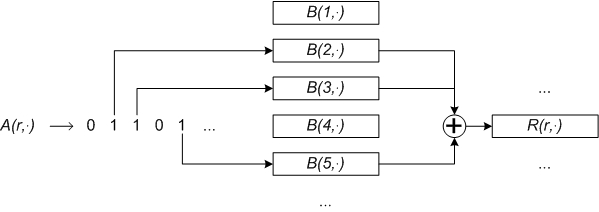
\includegraphics[width=\textwidth]{row_addition_method_deliberate_by_single_elements_scheme}}
	\caption{Схема процедуры умножения с анализом одного элемента.}
	\label{figures:RAM_DR_SEA_scheme}
\end{figure}

В данном случае достаточно простая процедура умножения, использующая строку $R(r,\cdot)$ в качестве
"аккумулятора"{} для частичной суммы, может иметь следующий вид:

\begin{program}{Избирательная процедура с анализом одного элемента}
	\programlabel{program:RAM_DR_SEA}
	\programline{1}{по всем r от 1 до $n$}
		\programline{2}{по всем c от 1 до $l$}
			\programline{3}{если $A(r,c)$ равен 1, то}
				\programline{4}{$R(r,\cdot) = R(r,\cdot) \oplus B(c,\cdot)$}
\end{program}

В данной процедуре управляющий фрагмент образован единственным условным оператором, сравнивающим текущий элемент
$A(r,c)$ с единицей, а вычисляющий фрагмент состоит из операции прибавления строки $B(c,\cdot)$
к строке $R(r,\cdot)$.

Если представить работу данной процедуры в виде хронологической последовательности действий
(рисунок~\ref{figures:RAM_DR_SEA_sequence}), то окажется, что она представляет собой
последовательность управляющих фрагментов У($c$), анализирующий элементы $A(r,c)$, которые прерываются вычисляющими
фрагментами В($c$), выполняющими прибавление строки $B(c,\cdot)$. 

\begin{figure}[h!]
	\center{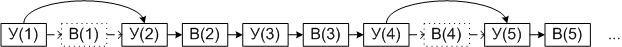
\includegraphics[width=\textwidth]{row_addition_method_deliberate_by_single_elements_sequence}}
	\caption{Последовательность действий процедуры с анализом одного элемента.}
	\label{figures:RAM_DR_SEA_sequence}
\end{figure}

После выполнения каждого управляющего фрагмента У($c$) требуется принимать решение о дальнейшем действии: требуется
либо выполнить вычисляющий фрагмент B($c$) (прибавить строку $B(c,\cdot)$), либо перейти к следующему управляющему
фрагменту У($c+1$) (рисунок~\ref{figures:RAM_DR_SEA_choice}). Постоянно возникающая необходимость
делать выбор --- выполнять прибавление строки $B(c,\cdot)$ или нет --- и связанная с ней неопределенность дальнейшей
последовательности действий в результате приводят к низкой эффективности процедуры умножения.

\begin{figure}[h!]
	\center{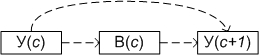
\includegraphics{row_addition_method_deliberate_by_single_elements_choice}}
	\caption{Выбор следующего действия.}
	\label{figures:RAM_DR_SEA_choice}
\end{figure}

\subsubsection { Анализ групп элементов } \label{subsubsection:RAM_DR_element_group_analysis}

Повысить эффективность избирательной процедуры умножения метода сложения строк можно путем "удлинения"{}
линейных участков и повышения "детерминированности"{} последовательности действий. Удлинение линейных участков
можно осуществить за счет переупорядочивания последовательности действий (
рисунок~\ref{figures:RAM_DR_SEA_reordering}):
сперва выполнять несколько управляющих фрагментов, проанализировав несколько элементов матрицы $A$, а затем выполнить несколько
соответствующих вычисляющих фрагментов, выполнив прибавление строк матрицы $B$.

\begin{figure}[h!]
	\center{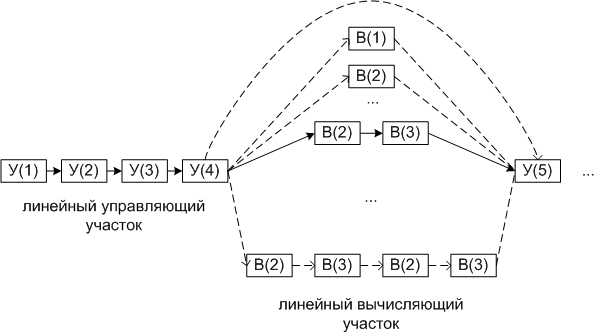
\includegraphics[width=\textwidth]{row_addition_method_deliberate_by_groups_of_elements_reordering}}
	\caption{Переупорядочивание управляющих и вычисляющих фрагментов.}
	\label{figures:RAM_DR_SEA_reordering}
\end{figure}

Переупорядочиванию управляющих и вычисляющих фрагментов соответствует обобщение анализа одного элемента матрицы
$A$ до анализа нескольких смежных элементов в количестве $k$.

Эффект переупорядочивания можно оценить следующим образом: если единицы в матрице $A$ встречаются с вероятностью $p$,
то среди $k$ элементов в среднем будет $p \cdot k$ единиц, и следовательно в среднем потребуется столько же $p \cdot k$
операций прибавления строки матрицы $B$, что безусловно позволит "удлинить"{} линейный участок, образованный
вычисляющими фрагментами, и повысить эффективность процедуры умножения.

Из приведенных соображений следует, что чем больше количество $k$, тем более длинным является линейный вычисляющий
участок и тем более эффективной является процедура умножения. Тем не менее, с ростом $k$ возрастает и сложность анализа $k$ смежных
элементов, в котором теперь необходимо сопоставлять группу из $k$ элементов одному из $2^k$ шаблонов (от $0 \dots 0$ до $1 \dots 1$)
и выбирать один из $2^k$ вариантов прибавления строк матрицы $B$.

В результате переупорядочивания изменяется схема работы процедуры умножения метода сложения строк, в частности для $k=4$ пример схемы
приведен на рисунке~\ref{figures:RAM_DR_EGA_scheme}.

\begin{figure}[h!]
	\center{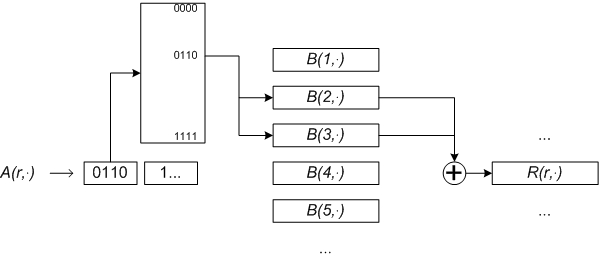
\includegraphics[width=\textwidth]{row_addition_method_deliberate_by_groups_of_elements_scheme}}
	\caption{Схема процедуры умножения с анализом $k=4$ элементов.}
	\label{figures:RAM_DR_EGA_scheme}
\end{figure}

Наиболее эффективными в данном случае по-видимому являются три следующих варианта процедуры умножения.

В первом варианте выполняется поиск шаблона, соответствующего группе элементов, на основе оператора выбора
(switch/case), реализованного в большом количестве языков программирования высокого уровня. В результате нахождения
шаблона, соответствующего группе элементов, управление передается в один из $2^k$ заранее составленных вычисляющих
фрагментов, реализующих прибавление соответствующих строк матрицы $B$.

\begin{program}{Избирательная процедура с анализом нескольких элементов: вариант с оператором выбора}
	\programlabel{program:RAM_DR_EGA_cases}
	\programline{1}{по всем r от 1 до $n$}
		\programline{2}{по всем c от 1 до $l$ с шагом $k$}
			\programline{3}{выбор для $A(r,c:c+k)$:}
			\programline{4}{при 0:}
				\programline{5}{// ничего не нужно прибавлять}
			\programline{4}{при 1:}
				\programline{5}{$R(r,\cdot) = R(r,\cdot) \oplus B(c,\cdot)$}
			\programline{4}{при 2:}
				\programline{5}{$R(r,\cdot) = R(r,\cdot) \oplus B(c+1,\cdot)$}
			\programline{4}{при 3:}
				\programline{5}{$R(r,\cdot) = R(r,\cdot) \oplus B(c,\cdot)$}
				\programline{5}{$R(r,\cdot) = R(r,\cdot) \oplus B(c+1,\cdot)$}
			\programline{4}{...}
			\programline{4}{при $2^k-1$:}
				\programline{5}{$R(r,\cdot) = R(r,\cdot) \oplus B(c,\cdot)$}
				\programline{5}{$R(r,\cdot) = R(r,\cdot) \oplus B(c+1,\cdot)$}
				\programline{5}{...}
				\programline{5}{$R(r,\cdot) = R(r,\cdot) \oplus B(c+k-1,\cdot)$}
\end{program}

Во втором варианте поиск шаблона, соответствующего группе элементов, выполняется на основе бинарного поиска (
с использованием операции сравнения '$<$'): сперва группа элементов сравнивается с шаблоном $10 \dots 0$, затем с
$11 \dots 0$ либо c $01 \dots 0$ и так далее. Для поиска шаблона, соответствующего группе из $k$ элементов,
потребуется произвести $k$ сравнений, после выполнения которых управление, как и в первом варианте, передается в один из
$2^k$ вычисляющих фрагментов, реализующих прибавление строк матрицы $B$.

\begin{program}{Избирательная процедура с анализом нескольких элементов: вариант с бинарным поиском (для $k=2$)}
	\programlabel{program:RAM_DR_EGA_binary_search}
	\programline{1}{по всем r от 1 до $n$}
		\programline{2}{по всем c от 1 до $l$ с шагом $2$}
			\programline{3}{если $A(r,c:c+k) < 10_2$, то}
				\programline{4}{если $A(r,c:c+k) < 01_2$, то}
					\programline{5}{// $00_2$ -ничего не нужно прибавлять}
				\programline{4}{иначе}
					\programline{5}{// $01_2$}
					\programline{5}{$R(r,\cdot) = R(r,\cdot) \oplus B(c,\cdot)$}
			\programline{3}{иначе}
				\programline{4}{если $A(r,c:c+k) < 11_2$, то}
					\programline{5}{// $10_2$}
					\programline{5}{$R(r,\cdot) = R(r,\cdot) \oplus B(c+1,\cdot)$}
				\programline{4}{иначе}
					\programline{5}{// $11_2$}
					\programline{5}{$R(r,\cdot) = R(r,\cdot) \oplus B(c,\cdot)$}
					\programline{5}{$R(r,\cdot) = R(r,\cdot) \oplus B(c+1,\cdot)$}
\end{program}

Наконец, в третьем варианте так же заранее формируются $2^k$ вычисляющих фрагментов, реализующих прибавление строк
матрицы $B$ в соответствии с $2^k$ шаблонами, и каждому фрагменту присваивается свой номер, двоичная запись которого
совпадает с шаблоном. Далее группа из $k$ элементов рассматривается как номер того фрагмента кода, который необходимо
выполнить для прибавления соответствующих строк матрицы $B$.

\begin{program}{Избирательная процедура с анализом нескольких элементов: вариант с подпрограммами}
	\programlabel{program:RAM_DR_EGA_pointer}
	\programline{1}{подпрограмма сложения \#1}
	\programline{1}{\{}
		\programline{2}{$R(r,\cdot) = R(r,\cdot) \oplus B(c,\cdot)$}
	\programline{1}{\}}

	\programline{1}{подпрограмма сложения \#2}
	\programline{1}{\{}
		\programline{2}{$R(r,\cdot) = R(r,\cdot) \oplus B(c+1,\cdot)$}
	\programline{1}{\}}

	\programline{1}{подпрограмма сложения \#3}
	\programline{1}{\{}
		\programline{2}{$R(r,\cdot) = R(r,\cdot) \oplus B(c+2,\cdot)$}
		\programline{2}{$R(r,\cdot) = R(r,\cdot) \oplus B(c+3,\cdot)$}
	\programline{1}{\}}

	\programline{1}{...}

	\programline{1}{подпрограмма сложения \#($2^k-1$)}
	\programline{1}{\{}
		\programline{2}{$R(r,\cdot) = R(r,\cdot) \oplus B(c,\cdot)$}
		\programline{2}{$R(r,\cdot) = R(r,\cdot) \oplus B(c+1,\cdot)$}
		\programline{2}{...}
		\programline{2}{$R(r,\cdot) = R(r,\cdot) \oplus B(c+k-1,\cdot)$}
	\programline{1}{\}}

	\programline{1}{по всем r от 1 до $n$}
		\programline{2}{по всем c от 1 до $l$ с шагом $k$}
			\programline{3}{вызов подпрограммы сложения \#$<A(r,c:c+k-1)>_2$}
\end{program}

Во всех трех вариантах требуется подготовка вычисляющих фрагментов в количестве $2^k$, что с ростом $k$ становится
отдельной трудоемкой задачей (например, при $k=8$ таких фрагментов уже 256), решать которую в конечном итоге
придется с привлечением автоматизированных средств генерации всех $2^k$ фрагментов кода.

Наиболее удачными значениями для количества $k$ элементов по-видимому следует признать степени числа 2 (2, 4, 8 и
так далее), поскольку элементы матрицы $A$ хранятся в виде бит байтов и выделение например 6 бит на границе двух байт
может оказаться настолько сложным, что может свести на нет все преимущества "удлинения"{} линейных участков.

В общем случае не имея экспериментальных данных сложно утверждать явное преимущество трех вариантов процедуры, основанной
на анализе нескольких элементов, над простейшей процедурой, использующей анализ одного элемента. С одной стороны процедура,
основанная на анализе нескольких элементов, имеет более длинные линейные участки, а с другой стороны требует более сложного
анализа элементов матрицы $A$, поэтому эффективность процедур, анализирующих несколько элементов, в основном определяется тем,
какой из двух факторов в результате оказывается "сильнее"{}.

Сложность анализа в каждом из рассмотренных выше трех вариантах процедуры с анализом нескольких элементов может оказаться
и не столь высокой.

В первом варианте используется "встроенный"{} оператор выбора, который с большой вероятностью транслируется
оптимизирующим компилятором в "быстрый"{} набор машинных инструкций.

Во втором варианте при анализе $k$ элементов требуется $k$ сравнений группы элементов и шаблона, и хотя эти
сравнения отличаются от сравнений одного элемента с единицей их количество такое же как и в реализации с анализом
одного элемента, которая последовательно анализирует $k$ элементов. Если сравнение группы элементов с шаблоном
реализовано "не очень сложно"{}, то сложность анализа в целом окажется не высокой.

В случае же третьего варианта последовательное сравнение $k$ элементов и вовсе заменено выборкой указателя
на вычисляющий фрагмент и вызова этого фрагмента по выбранному указателю.

Приведенные интуитивные соображения показывают, что во всех трех вариантах процедуры умножения, анализирующей несколько
элементов, анализ группы элементов может оказаться не столь сложным, и поэтому следует ожидать некоторый выигрыш от
"удлинения"{} линейных участков.

\subsection { Массовые процедуры умножения } \label{subsection:RAM_massive_routines}

Легко видеть, что в избирательных процедурах умножения управляющие фрагменты, выполняющие анализ групп элементов матрицы $A$,
чередуются с вычисляющими фрагментами, выполняющими прибавление строк матрицы $B$. Каким бы длинным (за
счет увеличения количества $k$) ни оказался фрагмент, выполняющий прибавление строк, рано или поздно он "прерывается"{} фрагментом,
 выполняющим анализ. Подобные "разрывы"{} в череде вычисляющих фрагментов по-прежнему порождают некоторую меру неопределенности,
связанную с тем, какой из вычисляющих фрагментов, выполняющий прибавление строк, будет выполнятся следующим, и как следствие становятся
 непреодолимым барьером на пути дальнейшего повышения эффективности избирательных процедур умножения.

Решение проблемы дальнейшего увеличения эффективности формулируется весьма просто: коль скоро управляющие фрагменты являются
препятствием на пути повышения эффективности, то от них необходимо избавиться, и оказывается существуют такие процедуры умножения,
в которых управляющие фрагменты заменены некоторым безусловным (выполняемым всегда) действием.

Рассмотрим вновь избирательную процедуру умножения с анализом одного элемента и представим, что управляющий фрагмент (проверка
условия равенства элемента $A(r,c)$ единице) отсутствует, а вместо него к строке матрицы $R$ всегда прибавляется
специальным образом модифицированные строки матрицы $B$: модифицированная строка является либо строкой из нулей, если элемент
$A(r,c)$ равен нулю, либо в точности повторяет строку матрицы $B$, если элемент $A(r,c)$ равен единице.

\begin{program}{Массовая процедура с анализом одного элемента}
	\programlabel{program:RAM_MR}
	\programline{1}{по всем r от 1 до $n$}
		\programline{2}{по всем c от 1 до $l$}
			\programline{3}{$R(r,\cdot) = R(r,\cdot) \oplus M ( B(c,\cdot); A(r,c) )$}
\end{program}

\noindent где $M$ --- функция модификации такая, что:
$$
M ( B(c,\cdot); e ) =
	\left \{
		\begin{array}{cc}
			0_{1 \times m}, & \text{если } e \text{ равен 0} \\
			B(c,\cdot), & \text{если } e \text{ равен 1}
		\end{array}
	\right .
,
$$
где $0_{1 \times m}$ --- строка из $m$ нулей.

Варианты организации модифицирующей функции $M$ могут быть весьма различными: варианты, в которых используется условный оператор
следует по-видимому считать неудачными, поскольку они фактически приводят к уже рассмотренной ранее избирательной процедуре
умножения с анализом одного элемента. Напротив, интерес представляют безусловные варианты, то есть не использующие условный
оператор.

В частности, одним из удачных безусловных вариантов является следующий:
\begin{equation}
	M ( B(c,\cdot); e ) = B(c,\cdot) \otimes e_{1 \times m},
	\label{equation:RAM_MR_modification_function}
\end{equation}

в которой $\otimes$ --- операция поэлементного умножения строк и $e_{1 \times m}$ --- строка,
все элементы которой равны $e$ (фактически значение $e$, "размноженное"{} на всю длину строки
матрицы $B$).

Схема работы массовой процедуры умножения с модифицирующей функцией~\ref{equation:RAM_MR_modification_function}
представлена на рисунке~\ref{figures:RAM_MR_scheme}: если значение $e$ равно
нулю, то строка $B(c,\cdot)$ поэлементно умножается на строку $0_{1 \times m}$, состоящую из нулей, и результатом
умножения является строка из нулей. Если же значение $e$ равно единице, то строка $B(c,\cdot)$ поэлементно умножается на
строку $1_{1 \times m}$, состоящую из единиц, и результатом умножения является исходная строка $B(c,\cdot)$. Далее
результаты всех умножений складываются между собой и размещаются в строке $R(r,\cdot)$. 

\begin{figure}[h!]
	\center{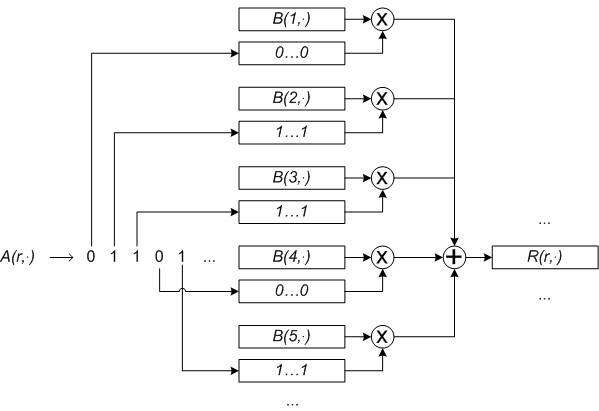
\includegraphics[width=\textwidth]{row_addition_method_massive_by_single_elements_scheme}}
	\caption{Схема массовой процедуры умножения.}
	\label{figures:RAM_MR_scheme}
\end{figure}

\section { Программные реализации }

\programreferencewithpage{program:RAM_DR_SEA}

\programreferencewithpage{program:RAM_DR_EGA_cases}

\programreferencewithpage{program:RAM_DR_EGA_binary_search}

\programreferencewithpage{program:RAM_DR_EGA_pointer}

\programreferencewithpage{program:RAM_MR}

Основные пути повышения эффективности (быстродействия)
\begin{enumerate}
	\item "удлинение"{} линейных участков,
\end{enumerate}

\begin{enumerate}
	\item векторизация,
	\item специализация
\end{enumerate}

\section{Вычислительная интенсивность}

В программной реализации 

\chapter{Метод четырех русских}

\section{Описание реализации}

\subsection{Параллельная часть}

Пусть требуется вычислить матрицу $R = A \otimes B$ (рисунок \ref{figures:FR:1}).

\begin{figure}
	\center{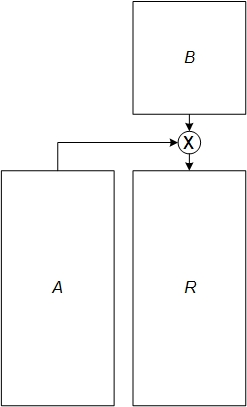
\includegraphics{four_russians_1}}
	\caption{Умножение $R = A \otimes B$.}
	\label{figures:FR:1}
\end{figure}

При наличии $P$ потоков матрица $B$ делится на блочные столбцы $B_1$, \ldots, $B_P$ (рисунок \ref{figures:FR:2}) так, чтобы в каждом блочном столбце $B_j$ оказалось
$k \in \{128, 256, 384, 512\}$ столбцов.

Поток с номером $j$ выполняет умножение всей матрицы $A$ на блочный столбец $B_j$ для получения блочного столбца $R_j = A \otimes B_j$.

\begin{figure}
	\center{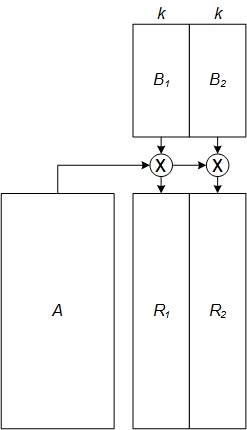
\includegraphics{four_russians_2}}
	\caption{Умножения $R_j = A \otimes B_j$ для $P = 2$ потоков.}
	\label{figures:FR:2}
\end{figure}

\subsection{Последовательная часть}

Для вычисления произведения $A \cdot B_j$ матрица $A$ делится на блочные столбцы $A_1$, \ldots, $A_{\frac{m}{128}}$ по 128 столбцов в каждом блочном столбце $A_i$, а блочный
столбец $B_j$ разбивается на блоки $B_{ij}$ по 128 строк в каждом (рисунки \ref{figures:FR:3} и \ref{figures:FR:4}), таким образом:
$$
	R_j = \bigoplus_{q=1}^{\frac{m}{128}} A_q \otimes B_{qj}
$$

\begin{figure}
	\center{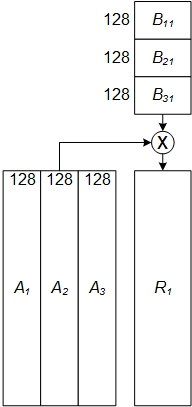
\includegraphics{four_russians_3}}
	\caption{Разбиение $A$ и $B_j$.}
	\label{figures:FR:3}
\end{figure}

\begin{figure}
	\center{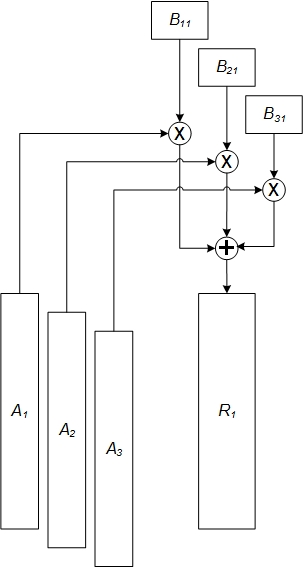
\includegraphics{four_russians_4}}
	\caption{Умножение блочных столбцов $A_q$ и блоков $B_qj$.}
	\label{figures:FR:4}
\end{figure}

Для вычисления отдельных произведений $A_q \otimes B_{qj}$ в строках $A_q$ элементы группируются по 4: в каждой строке $A_q$ ровно 128 элементов, поэтому всего в каждой строке
получается 32 группы по 4 элемента. Каждая группа из 4 элементов должна умножатся на соответствующие 4 строки в блоке $B_{qj}$, поэтому из строк блока $B_{qj}$ формируются
32 таблицы $T_{qj,1}$, \ldots, $T_{qj,32}$:
\begin{itemize}
	\item первая таблица $T_{qj,1}$ содержит всевозможные суммы 1-ой, 2-ой, 3-ой и 4-ой строк $B_{qj}$:
		$$
			\begin{array}{l}
				T_{qj,0} = 0, \\
				T_{qj,1} = B_{qj}(1,\cdot), \\
				T_{qj,2} = B_{qj}(2,\cdot), \\
				T_{qj,3} = B_{qj}(2,\cdot) \oplus B_{qj}(1,\cdot), \\
				T_{qj,4} = B_{qj}(3,\cdot) \\
				T_{qj,5} = B_{qj}(3,\cdot) \oplus B_{qj}(1,\cdot), \\
				T_{qj,6} = B_{qj}(3,\cdot) \oplus B_{qj}(2,\cdot), \\
				T_{qj,7} = B_{qj}(3,\cdot) \oplus B_{qj}(2,\cdot) \oplus B_{qj}(1,\cdot), \\
				\ldots \\
				T_{qj,15} = B_{qj}(4,\cdot) \oplus B_{qj}(3,\cdot) \oplus B_{qj}(2,\cdot) \oplus B_{qj}(1,\cdot), \\
			\end{array}
		$$
	\item вторая таблица $T_{qj,2}$ содержит всевозможные суммы 5-ой, 6-ой, 7-ой и 8-ой строк $B_{qj}$,
	\item \ldots
	\item 32-ая таблица $T_{qj,32}$ содержит всевозможные суммы 125-ой, 126-ой, 127-ой и 128-ой строк $B_{qj}$.
\end{itemize}

Для вычисления первой строки произведения $A_q \otimes B_{qj}$ рассматриваются 32 группы по 4 элемента в первой строке $A_q$ (рисунок \ref{figures:FR:5}). Первые 4 элемента
задают номер строки в первой таблице $T_{qj,1}$, вторые 4 элемента задают номер строки во второй таблице $T_{qj,2}$ и так далее для всех 32 таблиц. Выбранные из 32 таблиц
строки нужно сложить для получения первой строки $A_q \otimes B_{qj}$.

Аналогичную процедуру нужно повторить для вычисления всех остальных строк $A_q \otimes B_{qj}$.

\begin{figure}
	\center{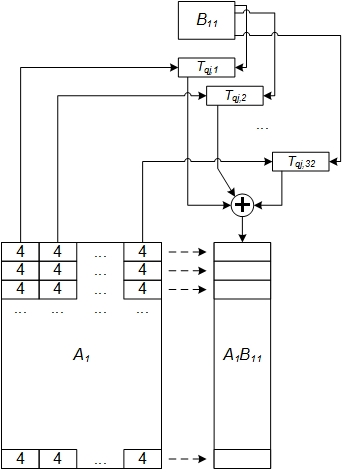
\includegraphics{four_russians_5}}
	\caption{Вычисление строк $A_1 \otimes B_{11}$ выборкой и сложением строк из таблиц.}
	\label{figures:FR:5}
\end{figure}

\end{document}
